\documentclass[12pt,a4paper]{article}
\usepackage[utf8]{inputenc}
\usepackage[brazil]{babel}
\usepackage{graphicx}
\usepackage{caption}
\usepackage{siunitx}
\usepackage{setspace}
\usepackage{float}
\usepackage[a4paper]{geometry}
\usepackage{amsmath,amsfonts,amstext,amscd,bezier}
\usepackage{mathtools}
\usepackage{amsthm}
\usepackage{mathrsfs}
\usepackage{times}
\usepackage{indentfirst}
\usepackage{hyperref}
\usepackage{placeins}
\usepackage{array}
\usepackage{subfigure}
\usepackage{wrapfig}
\usepackage{setspace}
\usepackage{gensymb}
\usepackage{svg}
\usepackage[backend=bibtex,sorting=none]{biblatex}
\usepackage{verbatim}
\usepackage[autostyle]{csquotes}
\usepackage{minted}
\linespread{1.1}

\begin{document}
	\begin{titlepage}
		\begin{center}
			\large Universidade de São Paulo\\[0.2cm]
			\large Instituto de Física de São Carlos\\[7cm]
			\huge \textbf{Relatório 1 - IntroFisComp}\\[6cm]
			
			\large Alexandre de Taunay Voloch \\[0.2cm]
		\end{center}
	\end{titlepage}

\section{Tarefa 1}

Essa tarefa simplesmente pede que calculemos as raízes rais de um polinômio simples da forma $ax^2+bx+c=0$. 

Para resolução, primeiro obtemos os valores de $a$, $b$ e $c$ do terminal e depois utilizamos o método de Bhaskara para encontrar os valores possíveis de $x$, e imprimimos de acordo com os resultados, contabilizando a possibilidade de haver só uma ou nenhuma raiz real.

\begin{minted}[
	mathescape,
	linenos,
	fontsize=\footnotesize,
	framesep=2mm,
	breaklines]
	{fortranfixed}
c     programa 1.1: bhaskara
      implicit real*8 (a-h,o-z)

      ! ler a, b, c
      write(*,*) "Insira a:"
      read(*,*) a
      write(*,*) "Insira b:"
      read(*,*) b
      write(*,*) "Insira c:"
      read(*,*) c

      delta = (b**2) - (4*a*c)

      if(delta.gt.0) then ! ver se delta é maior que 0
            x1 = ( -b + sqrt(delta) )/(2*a)
            x2 = ( -b - sqrt(delta) )/(2*a)
            write(*,*) "Duas raízes reais. x1=", x1, ", x2=", x2
      
      else if (delta.eq.0) then
            x = ( -b + sqrt(delta) )/(2*a)
            write(*,*) "Uma raiz real. x=", x

      else 
            write(*,*) "nenhuma raiz real"
      
      end if

      end

\end{minted}

Segue um exemplo de aplicação. Vamos inserir o polinômio $(x-2)(x-3) = x^2 - 5x +6 = 0$. Esperamos obter 2 e 3 como resposta.

\begin{minted}[
	mathescape,
	linenos,
	fontsize=\footnotesize,
	framesep=2mm,
	breaklines]
	{sh}
	./tarefa-1/tarefa-1.exe 
	 Insira a:
	1
	 Insira b:
	-5
	 Insira c:
	6
	 Duas raízes reais. x1=   3.0000000000000000      , x2=   2.0000000000000000  
\end{minted}

\section{Tarefa 2}
O problema pede para calcularmos a área do triângulo formado por dois vetores.

Esse problema é fácil de se resolver ao lembramos que o módulo do produto vetorial $\vec{v_1} \times \vec{v_2}$ é a área do paralelogramo formado por esses dois vetores. A área do triângulo será, portanto, simplesmente metade da área do paralelogramo.

\begin{minted}[
	mathescape,
	linenos,
	fontsize=\footnotesize,
	framesep=2mm,
	breaklines]
	{fortranfixed}
	!     programa: triangulo de 2 vetores
	      implicit real*8 (a-h,o-z)
	
	      write(*,*)"Insira x1, y1, z1, x2, y2, z2, um de cada vez:"
	      read(*,*)x1
	      read(*,*)y1
	      read(*,*)z1
	      read(*,*)x2
	      read(*,*)y2
	      read(*,*)z2
	
	      ! A área do triângulo é a mesma coisa que metade da área do paralelogramo
	      ! Que é a mesma coisa que o produto vetorial. Logo, vamos calcular o produto vetorial, no vetor v3 = v1 x v2
	
	      x3 = y1*z2 - z1*y2
	      y3 = z1*x2 - x1*z2
	      z3 = x1*y2 - x2*y1
	
	      v3 = sqrt( x3**2 + y3**2 + z3**2 ) ! Magnitude do vetor
	
	      area = v3 / 2
	      write(*,*)"A área do triângulo é", area
	
	      end
\end{minted}

Por exemplo, podemos testar para os vetores (1,0,0) e (0,1,0), que sabemos produzir um triângulo de área $\frac{1}{2}$.

\begin{minted}[
	mathescape,
	linenos,
	fontsize=\footnotesize,
	framesep=2mm,
	breaklines]
	{sh}
	./tarefa-2/tarefa-2.exe 
	 Insira x1, y1, z1, x2, y2, z2, um de cada vez:
	1
	0
	0
	0
	1
	0
	 A área do triângulo é  0.50000000000000000   
\end{minted}

\section{Tarefa 3}

O objetivo dessa tarefa é ordenar os primeiros m menores números de um arquivo de entrada, de tamanho desconhecido. Para resolvê-la, primeiro descobrimos o tamanho do arquivo de entrada (utilizando o comando end), e depois ordenamos a lista utilizando um algoritmo simples de ordenação (seria o equivalente ao selection sort.)

Perceba que nós apenas ordenamos os primeiros m menores números - ou seja, não precisamos ordenar a lista inteira, o que seria muito ineficiente, mas com nosso algoritmo conseguimos selecionar apenas tantos números quanto quisermos - essa é a vantagem de usar o selection sort nesse caso.

\begin{minted}[
	mathescape,
	linenos,
	fontsize=\footnotesize,
	framesep=2mm,
	breaklines]
	{fortranfixed}
      implicit real*8 (a-h,o-z)
      parameter (n_maximo_linhas=1000000)
      real*8 array_arquivo(n_maximo_linhas)
      open(unit=1, file='tarefa-3-entrada-1.in')

      do n=1,n_maximo_linhas
            read(1, *, end=200) a_linha
            array_arquivo(n) = a_linha
      end do
	
200   continue
      ! A última iteração do loop é quando ele sai do arquivo. Ou seja, o arquivo tem n-1 linhas
      n = n-1
      write(*,*) "Alcançamos o final do arquivo"
      write(*,*) "Numero de linhas N:", n
      close(1)

      write(*,*) "Insira M:"
      read(*,*) m

      ! agora vamos ordenar a lista
      do i=1,m
            a_menor = array_arquivo(i)
            i_posicao_menor = i
            ! O algoritmo de ordenar é o seguinte: Vamos passando pela lista, até encontrarmos uma linha
            ! que é menor do que a variável a_menor. assim, agora o menor valor é o dessa linha,
            ! e salvamos a posição dessa linha no i_posicao_menor.
            do j=i,n
                  if (a_menor.gt.array_arquivo(j)) then
                        a_menor = array_arquivo(j)
                        i_posicao_menor = j
                  end if
            end do
	
            ! no final de cada iteração, temos o menor número na lista de i até m. então,
            ! trocamos o número que está na posição i pelo verdadeiro menor número
	
            valor_antigo = array_arquivo(i)
            array_arquivo(i) = a_menor
            array_arquivo(i_posicao_menor) = valor_antigo
	
      end do
	
      ! agora vamos escrever no arquivo novo
      open(unit=2, file='tarefa-3-saida.dat')
      write(*,*) "M=", m
      write(2,*) "M=", m
      do i2=1,m
            write(*,*) array_arquivo(i2)
            write(2,*) array_arquivo(i2)
      end do
      close(2)
      end
\end{minted}

Os resultados são escritos no arquivo de saída, conforme pedido. Segue um exemplo para os primeiros 10 menores números do arquivo de entrada:

\begin{minted}[
	mathescape,
	linenos,
	fontsize=\footnotesize,
	framesep=2mm,
	breaklines]
	{sh}
	./tarefa-3.exe 
	 Alcançamos o final do arquivo
	 Numero de linhas N:      500000
	 Insira M:
	10
	 M=          10
	   1.2451782822608948E-006
	   5.5236741900444031E-006
	   6.6380016505718231E-006
	   6.6407956182956696E-006
	   7.6387077569961548E-006
	   7.8030861914157867E-006
	   1.0204501450061798E-005
	   1.0691117495298386E-005
	   1.1510215699672699E-005
	   1.2444797903299332E-005
	
\end{minted}

\section{Tarefa 4}

Nessa tarefa devemos encontrar os números primos até n e salvá-los em um arquivo. 

O algoritmo de encontrar números primos é bem simples. Utilizamos uma variável lógica que determina se um número é primo ou não. Inicialmente a variável é verdadeira. Fazemos um loop indo de $2$ até $(i-1)$ e verificamos se $i$ é divisível por algum número menor que ele (e maior que 1) - caso positivo, ele não é primo, e colocamos a variável como falsa e saímos do loop para evitar iterações desnecessárias. Por fim, caso a variável seja verdadeira após tudo isso, o número é primo, e salvamos ele no arquivo e imprimimos. Por final, também mostra-se o número total de primos.

\begin{minted}[
	mathescape,
	linenos,
	fontsize=\footnotesize,
	framesep=2mm,
	breaklines]
	{fortranfixed}
!     numeros primos 
      implicit real*8 (a-h,o-z)
      logical primo ! se um numero é primo ou não

      write(*,*) "Insira N:"
      read(*,*) n

      open(unit=1, file='tarefa-4-saida.dat') ! arquivo de saída

      ntotal = 0 ! n total de primos
      
      do i=2,n ! começo em 2 pq assumo que 1 não é primo
            primo = .true.
            do j=2,(i-1)
                  if (mod(i,j).eq.0) then ! se o numero nao tem resto de divisão por um numero menor que ele, ele não é primo
                        primo = .false.
			exit
!                  else if(j.eq.(i-1)) then ! Se j == n-1, significa que chegamos no final do loop, ou seja, i é primo!
!                        write(*,*) "primo"
!                        ntotal = ntotal + 1
                  end if
            end do
            if (primo) then
                  write(*,*) i, "primo"
                  write(1,*) i
                  ntotal = ntotal + 1
            end if
      end do

      write(*,*) "N total de primos:", ntotal
      write(1,*) "N total de primos:", ntotal

      close(1)

      end
\end{minted}

Dois exemplos. Primeiro, um que cabe na página - os números primos até 20:

\begin{minted}[
	mathescape,
	linenos,
	fontsize=\footnotesize,
	framesep=2mm,
	breaklines]
	{sh}
./tarefa-4.exe 
 Insira N:
20
           2 primo
           3 primo
           5 primo
           7 primo
          11 primo
          13 primo
          17 primo
          19 primo
 N total de primos:           8

\end{minted}

E agora os primos até 100000 (cem mil)

\begin{minted}[
	mathescape,
	linenos,
	fontsize=\footnotesize,
	framesep=2mm,
	breaklines]
	{sh}
(...)
       99961 primo
       99971 primo
       99989 primo
       99991 primo
 N total de primos:        9592

real    0m2,611s
user    0m1,389s
sys     0m0,016s

\end{minted}

Esse programa roda em menos de dois segundos (o comando time no linux mostra quanto tempo o programa realmente executou - 1,38 dos 2,61 segundos foram eu digitando o número 100000). Para testar, eu fiz um código com a mesma lógica de execução, só que no Python, para ver quanto tempo demora. Segue o código em Python (para motivos de demonstração)

\begin{minted}[
	mathescape,
	linenos,
	fontsize=\footnotesize,
	framesep=2mm,
	breaklines]
	{python}
n = int(input("Insira N:"))

ntotal = 0

for i in range(2, n+1):
    primo = True
    for j in range(2, i):
        if i%j == 0:
            primo = False
            break

    if primo:
        print(i, "primo")
        ntotal += 1

print("N total:", ntotal)
\end{minted}

Esse programa, com o mesmo input, demora mais de 50 segundos para rodar:

\begin{minted}[
	mathescape,
	linenos,
	fontsize=\footnotesize,
	framesep=2mm,
	breaklines]
	{sh}
(...)
99961 primo
99971 primo
99989 primo
99991 primo
N total: 9592

real    0m54,532s
user    0m53,252s
sys     0m0,020s
\end{minted}

Ou seja, fortran realmente é muito mais eficiente do que Python para cálculos numéricos. Achei bem interessante.

\section{Tarefa 5}
\subsection{a}

Aqui é pedido que aproximemos a função $ln(x)$ usando a sua série de Taylor para x entre 0 e 2. Devemos comparar nossa aproximação com a função intrínseca do Fortran $log(x)$ com uma precisão de $10^{-5}$.

O código é bem simples, apenas rodamos um loop para calcular cada iteração da série de Taylor e verificamos se a diferença entre os valores é menor do que a precisão desejada. Caso não seja, continuamos o loop.

\begin{minted}[
	mathescape,
	linenos,
	fontsize=\footnotesize,
	framesep=2mm,
	breaklines]
	{fortranfixed}
!     calcular lnx
      implicit real*8 (a-h,o-z)

      parameter (n_maximo_iteracoes=100000)
      parameter (precisao=1.d-5)

      write(*,*)"Insira x"
      read(*,*)x

      valor_correto = log(x)

      ! calcular usando série
      valor_aproximado = 0.d0

      do i=1,n_maximo_iteracoes
            valor_a_somar = ( (1-x)**i ) / i ! valor que vamos somar (na verdade subtrair) ao valor aproximado
            valor_aproximado = valor_aproximado - valor_a_somar

            difference = abs(valor_correto - valor_aproximado)
            if (difference.le.precisao) then
                  exit
            end if
      end do

      write(*,*)"valor aproximado obtido:", valor_aproximado
      write(*,*)"valor esperado (correto):", valor_correto
      write(*,*)"diferença entre os valores:", difference
      write(*,*)"iterações:", i

      end

\end{minted}

Seguem dois exemplos.

\begin{minted}[
	mathescape,
	linenos,
	fontsize=\footnotesize,
	framesep=2mm,
	breaklines]
	{sh}
./tarefa-5a/tarefa-5a.exe 
 Insira x
1.56
 valor aproximado obtido:  0.44467851544125125     
 valor esperado (correto):  0.44468582126144574     
 diferença entre os valores:   7.3058201944808943E-006
 iterações:          14

-------
./tarefa-5a/tarefa-5a.exe 
 Insira x
2
 valor aproximado obtido:  0.69313718065996721     
 valor esperado (correto):  0.69314718055994529     
 diferença entre os valores:   9.9998999780748221E-006
 iterações:       50000


\end{minted}

\subsection{b}

Aqui devemos modificar o código anterior para precisão dupla (no caso ele já estava) e comparar com a função $dlog(x)$ do Fortran, e encontrar o valor da precisão necessário para que ambas sejam equivalentes. 

Descobri que no Fortran os últimos dois dígitos de um número real são irrelevantes (floating point), flutuam arbitrariamente, então comparamos apenas os outros dígitos, que são 16 dígitos após o zero, o que nos deixa com uma precisão mínima de $\epsilon = 10^{-16}$.

\begin{minted}[
	mathescape,
	linenos,
	fontsize=\footnotesize,
	framesep=2mm,
	breaklines]
	{fortranfixed}
!     calcular lnx
      implicit real*8 (a-h,o-z)

      parameter (n_maximo_iteracoes=100000000)
      parameter (precisao=1.d-16)
      
      write(*,*)"Insira x"
      read(*,*)x
      !write(*,*)"Insira precisao"
      !read(*,*)precisao

      valor_correto = log(x)

      ! calcular usando série
      valor_aproximado = 0.d0

      do i=1,n_maximo_iteracoes
            valor_a_somar = ( (1-x)**i ) / i ! valor que vamos somar (na verdade subtrair) ao valor aproximado
            valor_aproximado = valor_aproximado - valor_a_somar

            difference = abs(valor_correto - valor_aproximado)
            if (difference.le.precisao) then
                  exit
            end if
      end do

      write(*,*)"valor aproximado obtido:", valor_aproximado
      write(*,*)"valor esperado (correto):", valor_correto
      write(*,*)"diferença entre os valores:", difference
      write(*,*)"iterações:", i

      end
\end{minted}

Segue um exemplo.

\begin{minted}[
	mathescape,
	linenos,
	fontsize=\footnotesize,
	framesep=2mm,
	breaklines]
	{sh}
./tarefa-5b/tarefa-5b.exe 
 Insira x
1.55
 valor aproximado obtido:  0.43825493093115525     
 valor esperado (correto):  0.43825493093115531     
 diferença entre os valores:   5.5511151231257827E-017
 iterações:          54

\end{minted}

\section{Tarefa 6}

Aqui é pedido para encontrarmos as raízes de uma equação de grau N complexa, $(z-2)^N = 3$. Aqui o problema é mais matemático do que de programação. Eu resolvi assim: fazemos $w = z-2$, logo $w^N = 3$. Usando a fórmula de Euler,

\[ w^N = 3 \Rightarrow \left(\rho e^{i\theta}\right) ^N = 3 = 3e^{i(0+2\pi k)} \Rightarrow\]

O que nos leva a

\[ \rho^N = 3 \Rightarrow \rho = \sqrt[N]{3} \]

\[ \theta = \frac{2\pi k}{N} \]

Onde $k = 0, 1, 2, ...., N-1$. 

Assim, encontramos o módulo e o ângulo de $w$, e encontramos z usando simplesmente que $z = w+2$ e passando para $w$ para a forma cartesiana.

Segue o programa:

\begin{minted}[
	mathescape,
	linenos,
	fontsize=\footnotesize,
	framesep=2mm,
	breaklines]
	{fortranfixed}

      implicit real*8 (a-h,o-z)
      double complex z
      
      pi = 4.d0*datan2(1.d0,1.d0) ! achei na internet esse jeito para ser exatamente pi
      write(*,*) "Insira N:"
      read(*,*) n

      rho = 3**(1/dble(n))
      do k=0,(n-1)
            theta = (2*dble(k))/dble(n)
            x_w = rho*dcos(theta*pi)
            y_w = rho*dsin(theta*pi)

            ! z = w+2
            x_z = x_w + 2
            y_z = y_w

            z = dcmplx(x_z, y_z)
            write(*,*)"k=",k
            write(*,*) "z=", z
      end do
      
      end
\end{minted}

Alguns exemplos:

\begin{minted}[
	mathescape,
	linenos,
	fontsize=\footnotesize,
	framesep=2mm,
	breaklines]
	{sh}
alex@G3-3590:~/projetos-fiscomp/projeto-1$ ./tarefa-6/tarefa-6.exe 
 Insira N:
1
 k=           0
 z=               (5.0000000000000000,0.0000000000000000)
alex@G3-3590:~/projetos-fiscomp/projeto-1$ ./tarefa-6/tarefa-6.exe 
 Insira N:
2
 k=           0
 z=               (3.7320508075688772,0.0000000000000000)
 k=           1
 z=        (0.26794919243112281,2.12115047744981358E-016)
alex@G3-3590:~/projetos-fiscomp/projeto-1$ ./tarefa-6/tarefa-6.exe 
 Insira N:
3
 k=           0
 z=               (3.4422495703074083,0.0000000000000000)
 k=           1
 z=               (1.2788752148462961,1.2490247664834064)
 k=           2
 z=              (1.2788752148462952,-1.2490247664834060)
alex@G3-3590:~/projetos-fiscomp/projeto-1$ ./tarefa-6/tarefa-6.exe 
 Insira N:
4
 k=           0
 z=               (3.3160740129524924,0.0000000000000000)
 k=           1
 z=               (2.0000000000000000,1.3160740129524924)
 k=           2
 z=        (0.68392598704750762,1.61172582740328218E-016)
 k=           3
 z=              (1.9999999999999998,-1.3160740129524924)
alex@G3-3590:~/projetos-fiscomp/projeto-1$ ./tarefa-6/tarefa-6.exe 
 Insira N:
5
 k=           0
 z=               (3.2457309396155174,0.0000000000000000)
 k=           1
 z=               (2.3849520307598664,1.1847605276718223)
 k=           2
 z=             (0.99218249943237513,0.73222227463044665)
 k=           3
 z=            (0.99218249943237491,-0.73222227463044642)
 k=           4
 z=              (2.3849520307598659,-1.1847605276718223)
alex@G3-3590:~/projetos-fiscomp/projeto-1$ ./tarefa-6/tarefa-6.exe 
 Insira N:
6
 k=           0
 z=               (3.2009369551760027,0.0000000000000000)
 k=           1
 z=               (2.6004684775880014,1.0400419115259520)
 k=           2
 z=               (1.3995315224119989,1.0400419115259520)
 k=           3
 z=        (0.79906304482399726,1.47072359813406007E-016)
 k=           4
 z=              (1.3995315224119982,-1.0400419115259518)
 k=           5
 z=              (2.6004684775880014,-1.0400419115259520)

\end{minted}

\section{Tarefa 7}
Aqui é pedido que calculemos o volume de uma esfera de $d$ dimensões usando o gerador de números aleatórios do Fortran, e depois comparar esse volume com o calculado analiticamente pela fórmula dada.

Eu fiz da seguinte forma. A função $rand()$ gera números entre 0 e 1, ou seja, no "primeiro quadrante" de um sistema de coordenadas cartesiano (de qualquer dimensão), onde cada $x_i > 0$ em um vetor. Logo, a fração de vetores que tiver seu módulo menor ou igual ao raio da esfera (no caso, 1, para simplificar) estará dentro do primeiro "quadrante" da esfera. Calculando essa fração (isto é, número de vetores dentro da esfera dividido pelo número total de vetores gerados) e multiplicando-a pelo volume de um cubo de lado 1 nesse primeiro quadrante (isto é, 1) nos dará o volume do primeiro quadrante da esfera.

Para descobrir o volume total da esfera, apenas extrapolamos usando o cubo. Uma esfera de raio 1 (i.e. diâmetro 2) será inteiramente contida em um cubo de lado 2 centrado na origem. O volume deste cubo será $2^d$. Portanto, o volume da esfera será $\frac{n_{dentro}}{n_{total}}\cdot 2^d$. Para $n_{total}$ suficientemente grande, isso deverá dar uma boa aproximação para o volume da esfera (considerando que a função $rand()$ gere vetores verdadeiramente aleatórios, isto é, distribuídos de forma isotrópica no espaço).

De fato, isso funciona. Depois, comparamos com o cálculo direto de $V_d$ usando a função $\Gamma$, que pode ser calculada recursivamente a partir dos valores dados. Segue o programa (o código imprime a porcentagem concluída):

\begin{minted}[
	mathescape,
	linenos,
	fontsize=\footnotesize,
	framesep=2mm,
	breaklines]
	{fortranfixed}

      implicit real*8 (a-h,o-z)
      parameter(iterations=10000000)
      integer d

      ! O algoritmo é o seguinte: calcular pontos aleatórios e ver quantos deles estão dentro ou fora da esfera 
      ! e calcular o volume a partir disso. como?
      ! Se vc esquematizar uma esfera de raio 1, em qualquer dimensão, ela será contida dentro de um cubo de raio 2
      ! centrado na origem (a esfera tem diâmetro 2.) Logo, calculamos primeiro a razão de pontos no primeiro quadrante
      ! (xi > 0) e depois extrapolamos isso para os outros quadrantes, calculando a partir do volume do cubo de 2^d.

      write(*,*)"Insira d (número de dimensões):"
      read(*,*)d

      volume_cubo = 2.e0**d

      n_dentro = 0

      do i=1,iterations
            distancia = 0.e0
            if (mod(i, iterations/10).eq.0) then
                  ! Imprimir a porcentagem concluída (para dimensões altas, o programa demora para rodar.)
                  n_porcento = i/(iterations/100)
                  !write(*,*) "porcentagem concluido:", n_porcento, "%"
            end if

            do j=1,d
                  xj = rand()
                  xj2 = xj**2.e0
                  distancia = distancia + xj2
            end do

            distancia = sqrt(distancia)

            if (distancia.le.1) then
                  n_dentro = n_dentro + 1
            end if
      end do

      razao_dentro = real(n_dentro)/real(iterations)
      volume_esfera = razao_dentro * volume_cubo
      write(*,*)
      write(*,*) "Volume da esfera: ", volume_esfera

      ! agora calcular usando gamma
      pi = 4.d0*datan2(1.d0,1.d0)

      ! precisamos ver se d é divisível por 2, pois assim sabemos qual versão da função gamma utilizar
      if (mod(d,2).eq.0) then
            gamma = 1.e0
            do i=1,int(d/2)
                  gamma = gamma * real(i)
            end do
      else
            gamma = sqrt(pi)
            do i=1,d,2 ! temos que fazer o do usando numeros inteiros senão o compilador reclama
                  ! (mesmo sendo que o fortran 77 permite números reais no do)
                  gamma = gamma * (i/2.e0) ! portanto precisamos dividir por 2 aqui
            end do
      end if

      v_calculado = (pi**(d/2.e0)) / gamma
      write(*,*)"Volume calculado com gamma:", v_calculado

      end
\end{minted}
Seguem exemplos para várias dimensões, comprovando os resultados esperados.

\begin{minted}[
	mathescape,
	linenos,
	fontsize=\footnotesize,
	framesep=2mm,
	breaklines]
	{sh}
alex@G3-3590:~/projetos-fiscomp/projeto-1/tarefa-7$ ./tarefa-7.exe 
 Insira d (número de dimensões):
1

 Volume da esfera:    2.0000000000000000     
 Volume calculado com gamma:   2.0000000000000000     
alex@G3-3590:~/projetos-fiscomp/projeto-1/tarefa-7$ ./tarefa-7.exe 
 Insira d (número de dimensões):
2

 Volume da esfera:    3.1418788433074951     
 Volume calculado com gamma:   3.1415926535897931     
alex@G3-3590:~/projetos-fiscomp/projeto-1/tarefa-7$ ./tarefa-7.exe 
 Insira d (número de dimensões):
3

 Volume da esfera:    4.1888313293457031     
 Volume calculado com gamma:   4.1887902047863914     
alex@G3-3590:~/projetos-fiscomp/projeto-1/tarefa-7$ ./tarefa-7.exe 
 Insira d (número de dimensões):
4

 Volume da esfera:    4.9345121383666992     
 Volume calculado com gamma:   4.9348022005446790     
alex@G3-3590:~/projetos-fiscomp/projeto-1/tarefa-7$ ./tarefa-7.exe 
 Insira d (número de dimensões):
5

 Volume da esfera:    5.2671136856079102     
 Volume calculado com gamma:   5.2637890139143249  
\end{minted}

\section{Tarefa 8}
\subsection{a}
Aqui precisamos simplesmente adaptar o programa original para fazer um loop indo até $d$, e colocando o output num arquivo. Não há muito o que explicar. Segue o programa:

\begin{minted}[
	mathescape,
	linenos,
	fontsize=\footnotesize,
	framesep=2mm,
	breaklines]
	{fortranfixed}

      implicit real*8 (a-h,o-z)
      parameter(iterations=10000000)
      integer d

      open(unit=1, file='tarefa-8-saida.dat')

      write(*,*)"Insira d (número de dimensões):"
      read(*,*)d
      write(*,*)"Insira r:"
      read(*,*)r

      pi = 4.d0*datan2(1.d0,1.d0)

      do n=1,d
            ! precisamos ver se d é divisível por 2, pois assim sabemos qual versão da função gamma utilizar
            if (mod(n,2).eq.0) then
                  gamma = 1.e0
                  do i=1,int(n/2)
                        gamma = gamma * real(i)
                  end do
            else
                  gamma = sqrt(pi)
                  do i=1,n,2 ! temos que fazer o do usando numeros inteiros senão o compilador reclama
                        ! (mesmo sendo que o fortran 77 permite números reais no do)
                        gamma = gamma * (i/2.e0) ! portanto precisamos dividir por 2 aqui
                  end do
            end if

            v_calculado = ((pi**(n/2.e0)) / gamma) * (r**real(n))
            write(*,*) n, v_calculado
            write(1,*) n, v_calculado
      end do

      end
\end{minted}

Por exemplo, para $d = 25$,

\begin{minted}[
	mathescape,
	linenos,
	fontsize=\footnotesize,
	framesep=2mm,
	breaklines]
	{sh}
./tarefa-8.exe 
 Insira d (número de dimensões):
25
 Insira r:
1
           1   2.0000000000000000     
           2   3.1415926535897931     
           3   4.1887902047863914     
           4   4.9348022005446790     
           5   5.2637890139143249     
           6   5.1677127800499694     
           7   4.7247659703314007     
           8   4.0587121264167676     
           9   3.2985089027387060     
          10   2.5501640398773451     
          11   1.8841038793898994     
          12   1.3352627688545893     
          13  0.91062875478328287     
          14  0.59926452932079188     
          15  0.38144328082330436     
          16  0.23533063035889312     
          17  0.14098110691713900     
          18   8.2145886611128191E-002
          19   4.6621601030088528E-002
          20   2.5806891390014051E-002
          21   1.3949150409020995E-002
          22   7.3704309457143478E-003
          23   3.8106563868521232E-003
          24   1.9295743094039221E-003
          25   9.5772240882317241E-004

\end{minted}

\subsection{b}
Da seção acima percebemos que o volume vai para zero conforme $d$ vai aumentando. Graficando isso conforme pedido (para r=0.9, 1.0, 1.1) temos:

\begin{figure}[H]
\centering
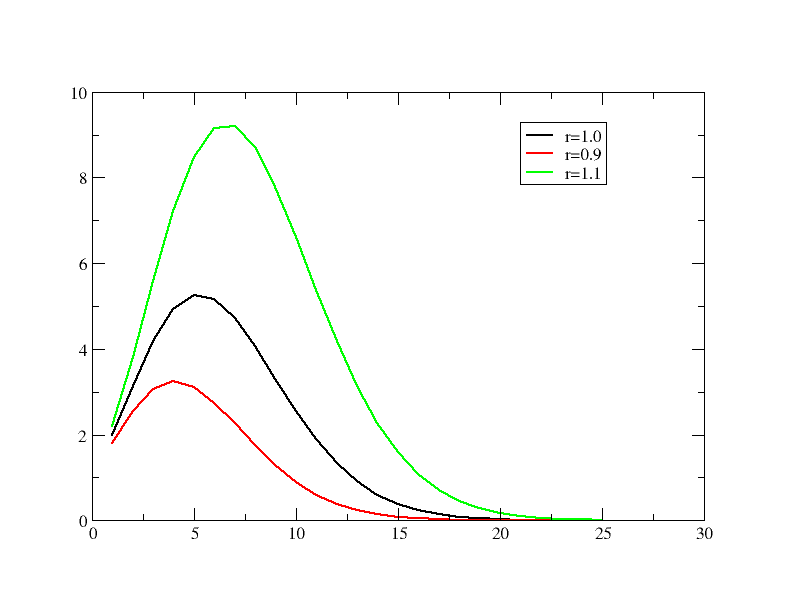
\includegraphics[width=\linewidth]{../tarefa-8-grafico}
\caption{Gráfico do volume de uma esfera em d dimensões para diferentes raios.}
\label{fig:tarefa-8-grafico}
\end{figure}

\section{Tarefa 9}

\subsection{a}
Aqui, está sendo pedido a razão entre o volume de um cubo de raio 1, em $d$ dimensões, e o volume de uma esfera na mesma dimensão. O volume do cubo é sempre 1. Logo, essa razão vale

\[ \frac{V_{cubo}}{V_{esfera}} = \frac{1}{V_{esfera}} = \frac{\Gamma(1 + d/2)}{\pi^{d/2}}\]

Como a função $\Gamma$, equivalente a uma função fatorial, cresce mais rápido do que $\pi^{d/2}$, o limite dessa razão para $d \Rightarrow \infty$ vale infinito.

\subsection{b}

Aqui temos que $1 \AA = 1\cdot10^{-10}m$, logo $1\AA^d = 10^{-10d}m^d$. Também $1 mm = 1\cdot10^{-3}m \Rightarrow 1 mm^d = 10^{-3d}m^d$.

A quantidade de átomos em um objeto é simplesmente o volume do objeto dividido pelo volume do átomo. Ou seja,

\[ n_a = \frac{10^{-10d}m^d}{10^{-3d}m^d} = 10^{7d} \]

Para $d=3$, isso nos dá $n_a=10^{28}$, que é uma aproximação razoável.

\end{document}